% !TEX TS-program = pdflatex
% !BIB TS-program = bibtex

\documentclass{ccjnl}

\usepackage[T1]{fontenc}
\usepackage{textcomp}
\usepackage{tabularx}
\usetikzlibrary{shapes.geometric,shapes,arrows.meta,positioning,fit,calc}
\renewcommand{\qedsymbol}{}

\title{System Relaxation for Resilient Network Governance: A Model-Driven Control Mechanism Against Structural Stress Concentration}


\def\publishmonth{5}
\def\publishyear{2026}

\begin{document}
\maketitle

\begin{abstract}
Prevailing network control strategies, rooted in static shortest-path logic, inherently suffer from ``stress concentration,'' where traffic excessively gravitates toward critical nodes, causing structural vulnerabilities and premature capacity saturation. While existing load-aware or AI-driven methods attempt to mitigate congestion through reactive pathfinding, they fail to address the underlying structural cause by neglecting to proactively control the network's cost landscape. To address this, we introduce the System Relaxation Algorithm (SRA), a model-driven supervisory governance layer inspired by physical relaxation that guides the network toward a “relaxed” emergent equilibrium of load balance. SRA functions as an interpretable ``white-box'' dynamical system where node costs evolve based on historically accumulated structural stress. By modeling discrete path switching as a non-smooth dynamical system, we provide rigorous proofs of global convergence and practical stability using piecewise Lyapunov functions, revealing that traditional static routing is merely a degenerate, memoryless case of this broader framework where system damping vanishes. Extensive simulations demonstrate that SRA's behavior is profoundly topology-dependent: in heterogeneous networks, it acts as a proactive performance optimizer, reducing peak centrality by over 80\% and increasing throughput by more than 45\%; in homogeneous topologies, it intelligently shifts its objective to resilience enhancement. SRA thus establishes a predictable, mathematically tractable paradigm for network governance that achieves an intelligent, topology-aware trade-off between performance and resilience.
\keywords{Network control; stress-aware governance; network resilience; self-organizing systems; load balancing; non-smooth dynamical systems; stability analysis}
\end{abstract}




\section{Introduction}
\label{sec:introduction}

Modern communication networks, from data center fabrics to large-scale ISP backbones, operate under increasingly volatile traffic conditions where stability is paramount. 
In such high-stakes environments, prevailing network control paradigms rooted in static shortest-path logic face a fundamental crisis. 
These traditional protocols inherently lack a mechanism for managing structural stress, leading to a phenomenon we term ``stress concentration''---a severe imbalance where load disproportionately gravitates toward a few critical topological bottlenecks.
This is not merely a transient congestion issue but a structural vulnerability: it creates ``stress singularities'' that render the network fragile to cascading failures and causes premature capacity saturation, where bottlenecks induce massive packet loss and soaring latency long before the network's physical capacity is reached.


\begin{figure}[t!]
    \centering
    % ---- (a) Before SRA ----
    \subfloat[Conventional Paradigm: Stress Concentration\label{fig:intro_before}]{%
    \begin{minipage}{0.46\columnwidth}
        \centering
        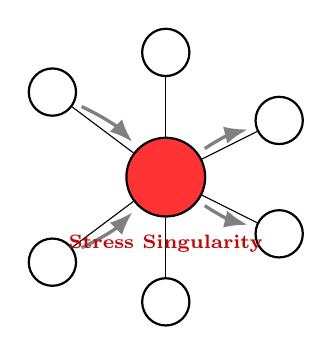
\begin{tikzpicture}[scale=0.72]
            \tikzstyle{node}=[circle, draw, thick, minimum size=6mm]
            \tikzstyle{hub}=[node, fill=red!80, minimum size=10mm]
            \tikzstyle{flow}=[-Latex, gray, thick, shorten <=1mm, shorten >=1mm]
            % Nodes
            \node[hub] (H) at (0,0) {};
            \node[node] (N1) at (2,1) {};
            \node[node] (N2) at (2,-1) {};
            \node[node] (N3) at (-2,1.5) {};
            \node[node] (N4) at (-2,-1.5) {};
            \node[node] (P1) at (0, 2.2) {};
            \node[node] (P2) at (0, -2.2) {};
            % Edges
            \draw (H) -- (N1); \draw (H) -- (N2);
            \draw (H) -- (N3); \draw (H) -- (N4);
            \draw (H) -- (P1); \draw (H) -- (P2);
            % Traffic Flows
            \draw[flow, line width=1.2pt] (N3) to [bend left=10] (H);
            \draw[flow, line width=1.2pt] (N4) to [bend right=10] (H);
            \draw[flow, line width=1.2pt] (H) to [bend left=10] (N1);
            \draw[flow, line width=1.2pt] (H) to [bend right=10] (N2);
            \node[below=0.1cm of H, text=red!80!black, font=\scriptsize\bfseries] {Stress Singularity};
        \end{tikzpicture}
    \end{minipage}
    }
    \hfill
    % ---- (b) After SRA ----
    \subfloat[SRA Control Paradigm: System Relaxation\label{fig:intro_after}]{%
    \begin{minipage}{0.46\columnwidth}
        \centering
        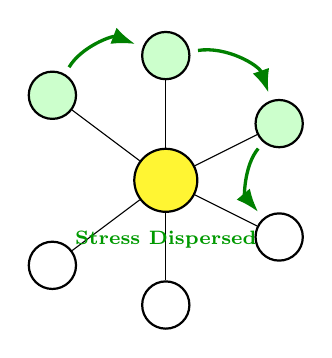
\begin{tikzpicture}[scale=0.72]
            \tikzstyle{node}=[circle, draw, thick, minimum size=6mm]
            \tikzstyle{hub}=[node, fill=yellow!80, minimum size=8mm]
            \tikzstyle{periph}=[node, fill=green!20]
            \tikzstyle{flow}=[-Latex, green!50!black, thick, shorten <=1mm, shorten >=1mm]
            % Nodes
            \node[hub] (H) at (0,0) {};
            \node[periph] (N1) at (2,1) {};
            \node[node] (N2) at (2,-1) {};
            \node[periph] (N3) at (-2,1.5) {};
            \node[node] (N4) at (-2,-1.5) {};
            \node[periph] (P1) at (0, 2.2) {};
            \node[node] (P2) at (0, -2.2) {};
            % Edges
            \draw (H) -- (N1); \draw (H) -- (N2);
            \draw (H) -- (N3); \draw (H) -- (N4);
            \draw (H) -- (P1); \draw (H) -- (P2);
            % Traffic Flows
            \draw[flow, line width=1.2pt] (N3) to [bend left=40] (P1);
            \draw[flow, line width=1.2pt] (P1) to [bend left=40] (N1);
            \draw[flow, line width=1.2pt] (N1) to [bend right=40] (N2);
            \node[below=0.1cm of H, text=green!60!black, font=\scriptsize\bfseries] {Stress Dispersed};
        \end{tikzpicture}
    \end{minipage}
    }
    
    \caption{Conceptual illustration of the core problem and the proposed SRA paradigm. SRA mitigates stress concentration by guiding the system toward a relaxed state of balanced load.}
    \label{fig:intro_scenario}
\end{figure}

The root of this fragility lies in a flawed focus on reactive symptoms rather than proactive structural governance. 
Prior work has largely attempted to patch this issue through two dominant approaches, yet both fall short of addressing the underlying cause:
\begin{itemize}
    \item \textbf{Reactive Load-Aware Routing (e.g., \cite{Macabale2020Cradle}):} These methods adjust paths based on transient metrics like queue length. They are essentially \textit{symptomatic treatments} that oscillate under high load due to delayed feedback loops.
    \item \textbf{Black-box AI Control (e.g., \cite{Wei2023GRLPS}):} While Deep Reinforcement Learning (DRL) agents can implicitly learn topology features, they function as uninterpretable ``black boxes,'' lacking the safety guarantees required for mission-critical infrastructure.
\end{itemize}

As summarized in Table~\ref{tab:related_work_comparison}, existing solutions fail to decouple structural stress from transient traffic state. They focus on \textit{pathfinding} within a fixed cost landscape, whereas the fundamental solution requires \textit{controlling the landscape itself}.

To bridge this gap, we propose a paradigm shift from reactive pathfinding to proactive \textit{stress governance}, inspired by the concept of ``relaxation'' in physical systems.
We introduce the System Relaxation Algorithm (SRA), a model-driven control system designed to disperse structural stress by dynamically reshaping the network's cost landscape.
Unlike black-box approaches, SRA operates as an interpretable, white-box dynamical system: it employs a ``leaky integrator'' mechanism to accumulate historical stress into a controllable state variable, thereby guiding the network toward an emergent equilibrium of load balance (as conceptually illustrated in Fig.~\ref{fig:intro_scenario}).
Crucially, this control paradigm aligns perfectly with Software-Defined Networking (SDN) architectures, leveraging the controller's global view to calculate stress and its centralized authority to enforce the resulting cost policies \cite{hou2020reliable}.

\begin{table*}[h!]
\centering
\caption{Taxonomy and Comparative Analysis of Network Control Paradigms}
\label{tab:related_work_comparison}
\renewcommand{\arraystretch}{1.3}
\small
\begin{tabularx}{\textwidth}{|l|X|X|X|X|}
\hline
\textbf{Feature} & \textbf{Reactive Load-Aware} & \textbf{Static Structural} & \textbf{AI-Driven / Learning} & \textbf{SRA (This Work)} \\
\hline \hline
\textbf{Sensing Object} & Instantaneous traffic (e.g., queue length, loss) & Static graph metrics (e.g., BC, degree) & High-dimensional patterns and graph features & \textbf{Accumulated structural stress ($S$)} \\
\hline
\textbf{Control Logic} & Symptomatic response to transient noise & Open-loop pathfinding on fixed weights & Black-box policy approximation (RL/GNN) & \textbf{Closed-loop model-driven dynamics} \\
\hline
\textbf{Mathematical Basis} & Heuristic cost functions & Graph theory and optimization & Statistical learning and inference & \textbf{Non-smooth dynamical systems} \\
\hline
\textbf{Stability Guarantee} & None (prone to oscillation and ping-pong effect) & N/A (Static/Open-loop) & Empirical (difficult to prove Lyapunov stability) & \textbf{Rigorous (Global attractivity \& Lyapunov decay)} \\
\hline
\textbf{Primary Goal} & Mitigate local, short-term congestion spikes & Average-case structural optimization & Maximize specific KPIs (throughput/delay) & \textbf{Disperse endemic structural stress} \\
\hline
\textbf{Deployment Mode} & Local / Distributed & Centralized (Offline) & Centralized (High-compute training) & \textbf{SDN-compatible (Model-driven)} \\
\hline
\textbf{Interpretability} & High & High & Low & \textbf{High (White-box Control Law)} \\
\hline
\end{tabularx}
\end{table*}

Our main contributions are summarized as follows:
\begin{enumerate}
    \item \textbf{A Unified Control-Theoretic Framework:} We formalize structural stress (via betweenness centrality) as a controllable state variable within a closed-loop dynamical system. \textbf{This framework explicitly decouples structural stress governance from low-level pathfinding}, treating conventional static routing as a degenerate case where the system's memory persistence (learning rate) is set to zero.
    
    \item \textbf{Rigorous Analysis of Discontinuous Dynamics:} We are the first to model the discrete path switching in centrality-based routing as a \textit{non-smooth dynamical system}. Using the theory of differential inclusions and piecewise Lyapunov functions, we provide formal proofs of global convergence and practical stability, ensuring the system is free from the destructive oscillations common in heuristic adaptive routing.
    
    \item \textbf{Topology-Dependent Intelligence:} Through extensive simulations, we demonstrate that SRA exhibits an emergent, topology-aware duality: in heterogeneous networks (e.g., Scale-free), it acts as a \textit{performance optimizer} by suppressing bottlenecks; in homogeneous networks (e.g., Random graphs), it automatically shifts to a \textit{resilience enhancement mechanism}, intelligently trading negligible latency for robust packet delivery.
\end{enumerate}

This work focuses on the algorithmic foundations and stability analysis of stress-aware network governance. 
While we discuss the alignment with SDN architectures, specific hardware implementations and south-bound protocol extensions are beyond the scope of this paper. The remainder of this paper is organized as follows: Section~\ref{sec:related_work} categorizes the existing literature and positions SRA within the routing landscape. 
Section~\ref{sec:model} establishes the unified theoretical framework, detailing the control-theoretic model, the rigorous stability analysis via non-smooth dynamics, and the formal bridge to capacity expansion. 
Section~\ref{sec:simulation} presents the empirical validation and analysis across the topological spectrum, and Section~\ref{sec:discussion_conclusion} concludes the paper.




\section{Related Work}
\label{sec:related_work}

The mitigation of structural stress remains a fundamental challenge at the intersection of network science and traffic engineering. While existing methodologies strive to balance traffic distribution, they vary significantly in their perception of network states and their subsequent control mechanisms. As synthesized in Table~\ref{tab:related_work_comparison}, there exists a discernible gap between traditional path-finding strategies and the active reshaping of a network's cost landscape. To situate the proposed System Relaxation Algorithm (SRA) within the broader research context, we categorize the existing literature into three distinct paradigms: reactive symptomatic management, static structural optimization, and black-box learning control.

\subsection{Reactive Control: Symptomatic Relief and Its Limitations}

The most pervasive paradigm in network control relies on \textit{reactive} feedback loops that adjust paths based on real-time performance metrics. These protocols typically monitor local queue lengths \cite{Macabale2020Cradle}, energy-aware load indicators \cite{SM2025Novel}, or composite link quality in highly dynamic satellite and vehicular environments \cite{Wang2025VANET, Fu2024SatelliteBC,wang2022cdmr}. For instance, the CRADLE protocol \cite{Macabale2020Cradle} leverages cross-layer cues to deflect traffic, while multi-criteria decision models \cite{Fouad2014MultiCriteria} and hierarchical cluster-based scaling \cite{Guizani2011Hierarchical} attempt to optimize routing decisions under fluctuating demands. Recent explorations in IoT and smart cities further extend this logic to position-based and occlusion-driven routing \cite{Darabkh2025SmartCity, Aditya2020ClosenessCluster}, addressing delays that often cascade across high-speed transport nodes \cite{Wu2024RailwayNode,ma2022traffic}.

While effective at mitigating immediate congestion, these methods essentially function as "symptom relievers" that address buffer overflows or link saturation rather than the underlying \textit{structural root causes}. By treating the network's cost landscape as an immutable constraint, reactive paradigms remain passive followers of instantaneous traffic noise. Consequently, they frequently suffer from the "ping-pong" effect—an instability where paths oscillate between overloaded and underloaded states due to delayed feedback. Lacking a long-term integration mechanism like SRA's leaky integrator, these approaches fail to distinguish between transient traffic spikes and endemic structural stress, and they lack the rigorous mathematical framework necessary to guarantee global stability under non-smooth traffic dynamics.

\subsection{Static Structural Optimization: The Open-Loop Governance Gap}

Recognizing the decisive role of network topology, a significant body of research leverages centrality metrics to guide routing and resource allocation. Betweenness Centrality (BC) and its sophisticated variants, such as link-variance optimization for optical networks \cite{Upadhyay2024OpticalBC} and weighted gravity models for multiplex systems \cite{Ni2023Gravity}, represent the established methodologies for identifying topological bottlenecks and influential nodes \cite{Basaras2019Influential, Wehmuth2021SpuriousPaths}. Theoretical advancements have further underscored that routing via quasi-shortest paths ($\rho$-geodesics) \cite{DeMedeiros2017QuasiShortest} or optimizing connectivity under probabilistic failures \cite{Cavallaro2022Connectivity} can significantly enhance network resilience. To circumvent the $O(N^3)$ computational complexity inherent in global centrality analysis, recent literature has proposed efficient approximation techniques, including hyperbolic space embeddings \cite{Stai2017Hyperbolic}, clustered parallelization \cite{Suppa2015FastBC}, and distributed estimation frameworks \cite{Maccari2020DistributedLoad, Maccari2018DistributedDV}. These structural insights have been applied across diverse domains, from optimizing SDN flow table storage \cite{Ma2019FlowTable} to enabling greedy forwarding in sparse networks \cite{Ahmed2025SparseNet} and energy-efficient path-finding in sensor networks \cite{Oliveira2010WSNcentrality}.

Despite their analytical depth, these structural optimization methods are fundamentally \textit{open-loop} and descriptive in nature. Even when accounting for temporal variations in centrality \cite{Ghanem2019DynamicCentrality}, the metrics are treated as passive observations rather than controllable state variables. Such strategies typically optimize for a static or "average" topology, failing to account for the non-linear "pressure accumulation" that occurs when real-world traffic flows interact with topological constraints. Unlike SRA, these approaches lack a rigorous control-theoretic feedback law to map structural observations into an adaptive cost landscape, leaving a "governance gap" between topological awareness and active congestion suppression.

\subsection{AI-Driven and Self-Organizing Control: The Black-Box Dilemma}

The recent surge in machine learning has catalyzed the deployment of Deep Reinforcement Learning (DRL) and Graph Neural Networks (GNNs) for complex network management. State-of-the-art agents, such as GRL-PS \cite{Wei2023GRLPS} and multi-agent GNN frameworks \cite{Feng2025MultiAgentGNN}, attempt to implicitly capture topological features to navigate intricate congestion scenarios. To mitigate the computational overhead of global metrics, some approaches utilize node embeddings to approximate traditional centrality measures \cite{Mendonca2021ApproxCentrality}. Parallel to these learning-based methods, bio-inspired self-organizing models \cite{Cheng2010SelfOrganizingModel, Guo2010HybridSelfOrg, Li2014PhysarumMulticast} and heuristic search strategies—including discrete particle swarm optimization \cite{Wang2019DPSO} and genetic algorithms \cite{Mu2024CarrierSelfOrg}—have been applied to dynamic cluster-based routing. These autonomous path-finding capabilities are particularly explored in mission-critical environments such as missile swarm networks \cite{Lu2022MissileSwarm,ma2021credibility}, where nodes must adapt to rapid topology changes.

Despite their empirical performance, these approaches frequently operate as \textit{black boxes} with opaque decision logic. They generally lack formal safety verification or rigorous Lyapunov stability guarantees, posing systemic risks to critical infrastructure where the unpredictable convergence of DRL agents remains a significant concern. Furthermore, heuristic and self-organizing models often overlook the non-smooth discontinuities inherent in discrete path-switching actions. This theoretical void is bridged by SRA, which provides a "white-box" alternative through the rigorous application of non-smooth dynamical systems theory, ensuring both mathematical explainability and guaranteed global convergence.

In summary, while the aforementioned paradigms have significantly advanced network engineering, a fundamental gap persists between topological awareness and active governance. Reactive methods prioritize speed over stability, static structural optimizations offer diagnostic depth but lack execution mechanisms, and learning-based controls trade mathematical explainability for empirical performance. Specifically, the networking community still lacks a unified framework that can bridge the "governance gap" between high-level structural observations (centrality) and low-level traffic control laws with guaranteed global stability. This paper addresses these limitations by introducing the System Relaxation Algorithm (SRA). By grounding the control logic in non-smooth dynamical systems theory and the "Cost Law" mechanism, SRA transitions the network management philosophy from passive path-finding to the active, stable, and explainable reshaping of the network's cost landscape.

\section{Theoretical Model and Methods}
\label{sec:model}

We formulate the problem of stress-aware network governance not as a sequence of heuristic routing updates, but as a \textbf{discrete-time, non-smooth dynamical system}. 
This control-theoretic perspective is decisive: it allows us to transcend the stability pitfalls of naive reactive protocols, which often collapse into destructive oscillations due to their lack of system memory.
In our framework, the network's cost landscape is no longer a static input, but a dynamic state variable governed by a physics-inspired ``leaky integrator.''
This section provides a systematic construction of this system. 
We first define the network model and formalize structural stress as a controllable state. 
We then detail the core state evolution law that couples continuous stress accumulation with discrete path switching. 
The culmination is a rigorous analysis using piecewise Lyapunov functions and discrete-time inclusion theory, proving that SRA guarantees global convergence to a robust equilibrium---a theoretical guarantee that heuristic methods fundamentally lack.

\subsection{Network Model and Load Metric}

We model the underlying network topology as a connected undirected graph $G=(V,E)$ with $N=|V| \ge 3$ nodes. 
From a control perspective, the network's ``plant'' is governed by a dynamically evolving node cost vector $C \in \mathbb{R}^N_+$. 
This vector defines the instantaneous \textit{cost landscape}, where the cost of any path $P$ is the sum of the transit costs of its constituent nodes, i.e., $d(P) = \sum_{v \in P} C_v$. 
Traffic flows are assumed to follow lowest-cost paths within this landscape.

To quantify the structural stress induced by a specific cost distribution, we employ \textbf{Betweenness Centrality (BC)} as the primary feedback signal. 
The unnormalized stress on node $i$, denoted $\kappa_i(S)$, represents its absolute topological load:
\begin{equation}
    \label{eq:bc_definition}
    \kappa_i(S) = \sum_{s\neq i\neq t\in V} \frac{\sigma^{\,C(S)}_{st}(i)}{\sigma^{\,C(S)}_{st}}
\end{equation}
where $\sigma^{\,C(S)}_{st}$ is the total number of shortest paths between $s$ and $t$ under the cost configuration $C(S)$, and $\sigma^{\,C(S)}_{st}(i)$ is the subset passing through $i$.

Since $\kappa_i(S)$ is unbounded, we project this feedback signal into a compact state space to ensure system stability. 
We define the max-normalized stress vector as:
\begin{equation}
    \label{eq:bc_normalization}
    \kappa_{\max}(S):=\max_j\kappa_j(S).
\end{equation}
\begin{equation}
    \mathrm{norm}(\kappa(S)) =
    \begin{cases}
    \displaystyle \frac{\kappa(S)}{\kappa_{\max}(S)}, & \text{if } \kappa_{\max}(S) > 0,\\[6pt]
    \mathbf{0}, & \text{otherwise.}
    \end{cases}
\end{equation}
This normalization confines the feedback signal strictly within the unit hypercube $[0,1]^N$. 
\textbf{Key Geometric Property:} Crucially, for any finite graph with a deterministic tie-breaking rule, the set of all possible shortest-path configurations is finite. 
This implies that $\mathrm{norm}(\kappa(S))$ does not vary continuously but jumps between a \textbf{finite set of constant vectors}. 
This quantization is non-trivial; it renders the system dynamics \textit{piecewise constant}, forming the topological foundation for our non-smooth convergence analysis in Section~\ref{sec:convergence_analysis}.

% --- 这是 Fig. 2 的完整代码 ---
\begin{figure*}[t!]
    \centering
    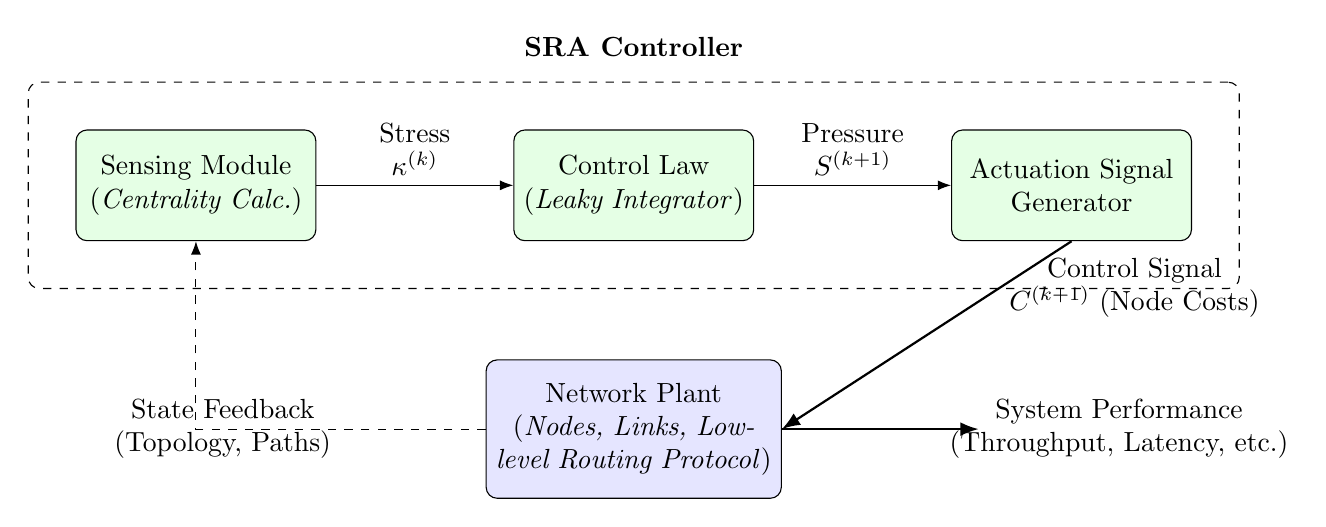
\begin{tikzpicture}[
        auto,
        node distance=1.5cm and 2.5cm,
        plant/.style={rectangle, draw, fill=blue!10, text width=10em, text centered, rounded corners, minimum height=5em},
        module/.style={rectangle, draw, fill=green!10, rounded corners, text width=8em, text centered, minimum height=4em},
        line/.style={draw, -{Latex}},
        signal/.style={draw, -{Latex}, thick},
        feedback/.style={draw, -{Latex}, dashed}
    ]
    % SRA Controller's Internal Modules
    \node [module] (sensing) {Sensing Module \\ (\textit{Centrality Calc.})};
    \node [module, right=of sensing] (law) {Control Law \\ (\textit{Leaky Integrator})};
    \node [module, right=of law] (actuation) {Actuation Signal Generator};
    % Network Plant
    \node [plant, below=of law] (plant) {Network Plant \\ (\textit{Nodes, Links, Low-level Routing Protocol})};
    % Dashed container for the SRA controller
    \node [draw, rounded corners, fit=(sensing) (law) (actuation), label={[yshift=0.2cm]above:\textbf{SRA Controller}}, inner sep=0.6cm, dashed] (controller_box) {};
    % Connections
    \path [signal] (actuation.south) -- node [right, pos=0.25, align=center] {Control Signal \\ $C^{(k+1)}$ (Node Costs)} (plant.east);
    \path [feedback] (plant.west) -| node [left, pos=0.25, align=center] {State Feedback \\ (Topology, Paths)} (sensing.south);
    % Internal Controller Connections
    \path [line] (sensing.east) -- node [above, align=center] {Stress \\ $\kappa^{(k)}$} (law.west);
    \path [line] (law.east) -- node [above, align=center] {Pressure \\ $S^{(k+1)}$} (actuation.west);
    % System Performance Output
    \coordinate[right=of plant] (output_coord);
    \path [signal] (plant.east) -- node [right, pos=0.8, align=center] {System Performance \\ (Throughput, Latency, etc.)} (output_coord);
    \end{tikzpicture}
    \caption{The architecture of the SRA as a closed-loop control system. The SRA controller acts as a supervisory layer that governs the underlying network plant by dynamically adjusting the cost landscape.}
    \label{fig:sra_architecture}
\end{figure*}

\subsection{SRA: Core Mechanism and Algorithm Implementation}
\label{subsec:sra_mechanism}

\textit{Design Philosophy: SRA as a Supervisory Layer.} 
Crucially, SRA is not a routing protocol designed for packet forwarding; rather, it functions as a supervisory governance layer that optimizes the network's ``cost landscape.'' It provides an adaptive metric space upon which standard routing protocols (e.g., OSPF, IS-IS, or Dijkstra) can then execute without triggering structural bottlenecks.

Having established the state space, we now derive the \textit{laws of motion} for the SRA controller. 
We formally architect SRA not merely as a routing algorithm, but as a \textbf{closed-loop feedback control system}, as visualized in Fig.~\ref{fig:sra_architecture}. 
The central design philosophy is to decouple the instantaneous observation of stress from the immediate actuation of costs. 
By inserting a temporal integration stage---specifically, a \textbf{leaky integrator}---between sensing and actuation, the SRA controller governs the underlying network plant with a critical damping effect. 
This design fundamentally distinguishes SRA from ``amnesic'' reactive protocols, allowing it to filter out high-frequency transient noise and respond only to persistent structural trends.



A naive feedback mechanism that sets node costs directly proportional to instantaneous centrality is inherently unstable, creating a ``bang-bang'' control regime that leads to persistent, destructive oscillations. 
To ensure rigorous stability, SRA's design must incorporate system memory to dampen these high-frequency fluctuations. 
We achieve this using an Integral (I) control structure, implemented as a \textbf{leaky integrator}. 
We define a core state vector, the ``accumulated pressure'' $S \in \mathbb{R}^N_+$, which represents the historically integrated stress on each node. 
This state evolves according to the discrete-time transition equation:
\begin{equation}
    \label{eq:pressure_update}
    S_i^{(k+1)} = (1 - \alpha) S_i^{(k)} + \alpha \cdot \mathrm{norm}(\kappa_i^{(k)})
\end{equation}
where $k$ is the iteration step and the learning rate $\alpha \in (0,1)$ governs the system's memory persistence. 
Physically, this equation functions as a \textbf{digital low-pass filter}: the $(1-\alpha)$ term provides a critical \textbf{damping} effect, allowing the system to absorb transient traffic shocks while tracking persistent structural trends.

\begin{remark}[Relationship to Reactive Routing]
\label{rem:reactive_routing}
It is critical to observe that standard reactive routing protocols correspond to a \textit{degenerate case} of Eq.~\eqref{eq:pressure_update} where $\alpha=1$. 
\end{remark}

In this memoryless limit, the damping term vanishes ($1-\alpha=0$), explaining why such protocols inherently lack stability under high load.

The node transit cost $C$, the system's actuation signal, is then defined as an affine control law based on this stable historical state:
\begin{equation}
    \label{eq:cost_update}
    C_i^{(k+1)} = 1 + \beta_I \cdot S_i^{(k+1)}
\end{equation}
where $1$ is the base physical cost and $\beta_I > 0$ is the ``pressure-to-cost'' gain factor. 
By deriving costs from the system's history ($S$) rather than instantaneous noise, SRA makes stable, proactive decisions.

% --- Fig. 3 Code Remains Unchanged ---
\begin{figure}[hbtp]
    \centering
    \includegraphics[width=0.9\columnwidth]{fig3xunhuan.eps}
    \caption{The iterative workflow of the SRA control loop, illustrating the four key phases of sensing, decision-making, actuation, and system influence that drive the network toward a state of dispersed structural stress.}
    \label{fig:sra_workflow}
\end{figure}

The complete iterative process is formalized in Algorithm~\ref{alg:sra}, and its cyclical workflow is visualized in Fig.~\ref{fig:sra_workflow}. 
To address the non-smooth nature of discrete path switching, the algorithm introduces a \textit{stabilization constraint}: the minimum dwell time $T_d$. 
This mechanism prevents the system from reacting to the immediate perturbations caused by its own control actions, allowing the network state to settle before the next update.
The core principle of SRA is to fundamentally reshape the network's ``cost landscape'' based on accumulated structural stress. 
As shown conceptually in Fig.~\ref{fig:sra_mechanism_visualization}, this forces the routing protocol to intelligently trade path efficiency for bottleneck avoidance, rerouting traffic from a physically short but high-stress path to a longer but more stable peripheral route.

% --- 这是 Algorithm 1 的完整代码 ---
\begin{breakablealgorithm}
\caption{System Relaxation Algorithm (SRA)}
\label{alg:sra}
\begin{algorithmic}[1]
\REQUIRE Graph $G=(V,E)$; learning rate $\alpha \in (0,1)$; pressure-cost factor $\beta_I > 0$; stopping threshold $\varepsilon > 0$; max iterations $K_{\max}$; optional min dwell time $T_d \ge 1$.
\ENSURE Final node cost vector $C^{(k+1)}$ and the corresponding routing policy.
\STATE Initialize $S^{(0)} \leftarrow \mathbf{0}$ and $C^{(0)} \leftarrow \mathbf{1}$.
\FOR{$k=0,1,2,\ldots,K_{\max}-1$}
\STATE Compute all-pairs shortest paths using node costs $C^{(k)}$.
\STATE Compute unnormalized centrality $\kappa^{(k)}$ based on new paths.
\STATE Update pressure: $S^{(k+1)} \leftarrow (1-\alpha)S^{(k)}+\alpha\,\mathrm{norm}(\kappa^{(k)})$.
\STATE Update cost: $C^{(k+1)} \leftarrow 1+\beta_I\,S^{(k+1)}$.
\IF{a path set switch occurred at $k$ and $T_d > 1$}
\STATE Use the current path set for the next $T_d-1$ steps, executing only the evaluation and convergence checks.
\ENDIF
\IF{$\|S^{(k+1)}-S^{(k)}\|_\infty \le \varepsilon$ and the path set is stable}
\STATE \textbf{break}
\ENDIF
\ENDFOR
\end{algorithmic}
\end{breakablealgorithm}

% --- 这是 Fig. 4 (原文fig 7) 的代码 ---
\begin{figure}[t!]
    \centering
    % Ensure the file path to your PDF is correct
    \includegraphics[width=0.8\columnwidth]{figure_7_microscopic_path_change.eps}
    \caption{A conceptual visualization of SRA's path reshaping mechanism. The algorithm diverts traffic from the efficient but congested 2-hop path (red dashed) through the central hub to a longer but more stable 4-hop peripheral path (green solid).}
    \label{fig:sra_mechanism_visualization}
\end{figure}

\subsection*{Complexity and Scalability Analysis}

The computational complexity of the baseline SRA iteration is governed by the exact centrality calculation, scaling as $O(N(E + N \log N))$ using Brandes' algorithm. 
While this overhead is acceptable in centralized SDN deployments due to the separation of control-plane computation and data-plane forwarding, SRA also supports a \textbf{distributed sensing mode} for massive-scale networks.
In this mode, we relax the requirement for exact global calculation. 
Instead, individual nodes act as distributed estimators: they approximate their own local centrality by tracking the cardinality of unique source-destination pairs in transiting flows. 
These local stress indicators are then efficiently aggregated via standard management protocols (e.g., OSPF-TE extensions or SDN In-band Network Telemetry), effectively reducing the computational complexity to $O(1)$ per node.
This hybrid architecture ensures that SRA remains scalable and deployable, transitioning seamlessly from exact structural analysis in small/medium networks to statistical approximation in hyper-scale environments.


\subsection{Theoretical Analysis of Model Convergence}
\label{sec:convergence_analysis}

We now establish the rigorous mathematical foundation for the SRA control loop. 
The central analytical challenge lies in the system's hybrid nature: the continuous evolution of pressure states ($S$) is coupled with the discrete, discontinuous switching of routing topologies. 
This non-smoothness renders standard gradient-based control theory inapplicable and represents the primary theoretical barrier where heuristic protocols fail to guarantee stability.

To overcome this, we model the system dynamics using the formalism of discrete-time differential inclusions. 
Our analysis proceeds in three logical steps to construct a complete stability proof:
\begin{enumerate}
    \item \textbf{Global Attractivity (Safety):} We first prove the existence of a global attractor, guaranteeing that system trajectories are strictly confined within a bounded safety region and never diverge.
    \item \textbf{Lyapunov Decay (Energy):} We construct a specialized \textit{piecewise Lyapunov function} to quantify the system's ``structural energy,'' proving that the feedback loop dissipates stress according to a strict contraction mapping.
    \item \textbf{Practical Stability (Engineering):} Finally, we formalize the minimum dwell time $T_d$ not as a heuristic parameter, but as a necessary condition to eliminate high-frequency chattering (Zeno behavior), deriving an explicit convergence rate to a stable $\varepsilon$-neighborhood.
\end{enumerate}



\subsection{Global Attractiveness and Existence Guarantee for Convergence}
\label{subsec:attractivity}

The convergence analysis of centrality-based routing is notoriously difficult due to the piecewise constant, non-smooth nature of the map $\kappa(S)$. 
Heuristic approaches often ignore the discontinuities caused by path switching, leading to theoretical vacuums.
To establish a rigorous guarantee, we do not merely approximate the system; we \textbf{regularize} the hybrid dynamics into a \textbf{discrete-time differential inclusion}. 
The update rule is formalized as the set-valued map:
\begin{equation}\label{eq:inclusion_map}
S^{(k+1)} \in F(S^{(k)}) := (1-\alpha)S^{(k)}+\alpha\,\mathcal{N}(S^{(k)})
\end{equation}
where $\mathcal{N}(S)$ is the \textbf{Krasovskii regularization} of the discontinuous mapping $\mathrm{norm}(\kappa(\cdot))$. 
Geometrically, this operation takes the convex hull of all limit points in a vanishing neighborhood of $S$, effectively ``filling in the gaps'' caused by discrete routing decisions (e.g., tie-breaking). 
This yields a mathematically well-behaved map, allowing us to derive the following foundational properties.

\begin{lemma}[Global Confinement and Safety]
\label{lemma:invariance}
Let the state space be the unit hypercube $X=[0,1]^N$. 
The discrete-time inclusion for SRA, given by $S^{(k+1)}\in F(S^{(k)})$, is strictly confined within $X$. 
Proof formally, $X$ is a \textbf{compact, positively invariant set} and serves as a compact absorbing set.
\textit{Physical Interpretation:} This lemma guarantees that the structural stress never diverges to infinity; the system possesses an intrinsic ``safety boundary'' dictated by the normalization mechanism.
\end{lemma}
\begin{proof}[Proof Sketch]
The proof demonstrates that if a state $S^{(k)}$ resides within the hypercube $X$, its successor $S^{(k+1)}$---being a convex combination of elements in $X$---must inherently remain within $X$. This geometric property establishes positive invariance. \textit{The full formal proof is provided in Appendix~\ref{app:proof_lemma_invariance}.}
\end{proof}

With safety guaranteed, we verify the topological regularity of the control map.

\begin{proposition}[Topological Regularity]
\label{prop:usc}
The set-valued map $F(\cdot)$ defined in \eqref{eq:inclusion_map} is \textbf{Upper Semi-Continuous (USC)} with \textbf{non-empty, compact, and convex} values.
\end{proposition}
\begin{proof}[Proof Sketch]
The proof exploits the piecewise constant structure of $\mathcal{N}(S)$, which stems from the finite nature of the network's path configurations (see Section~\ref{sec:model}-A). This structure ensures that the graph of the map is closed, a sufficient condition for the USC property in bounded spaces. \textit{The full formal proof is provided in Appendix~\ref{app:proof_prop_usc}.}
\end{proof}

Combining the global confinement (Lemma~\ref{lemma:invariance}) with topological regularity (Proposition~\ref{prop:usc}), we establish the system's ultimate destiny.

\begin{theorem}[Universal Convergence to Equilibrium]
\label{thm:attractor}
For the discrete-time inclusion \eqref{eq:inclusion_map}, there exists a non-empty, compact, and positively invariant set $\Omega\subset X:=[0,1]^N$, termed the \textbf{Global Attractor}, such that for any initial configuration $S^{(0)}\in X$:
\begin{equation}\label{eq:attractor_convergence}
\mathrm{dist}\big(S^{(k)},\Omega\big)\ \to\ 0\qquad (k\to\infty).
\end{equation}
\end{theorem}
\begin{proof}[Proof Sketch]
The proof leverages the theory of dynamical systems on compact metric spaces. Since the trajectory is pre-compact (due to Lemma~\ref{lemma:invariance}) and governed by a USC map (Proposition~\ref{prop:usc}), its $\omega$-limit set is non-empty and quasi-invariant. The union of all such limit sets constitutes the global attractor $\Omega$. \textit{The full formal proof is provided in Appendix~\ref{app:proof_thm_attractor}.}
\end{proof}

Theorem~\ref{thm:attractor} is definitive: it guarantees that SRA will never exhibit unbounded divergence. The network state is mathematically forced to evolve toward a stable, bounded region $\Omega$---the theoretical manifestation of the ``relaxed'' state.

\subsection{Energy Dissipation and Bounded Oscillation Analysis}
\label{subsec:lyapunov}

While the existence of a global attractor guarantees safety, it does not quantitatively preclude persistent oscillations (chattering). 
To rigorously characterize the system's steady-state dynamics, we introduce a specialized analytical tool from non-smooth mechanics: the \textbf{piecewise Lyapunov function}.
We construct a scalar function $V(S)$ to quantify the system's ``structural potential energy''---defined as the squared Euclidean distance from the current state to the ideal equilibrium set of the instantaneous topology.
Formally:
\begin{equation}\label{eq:lyapunov_def}
V(S):=\min_{c\in\mathcal N(S)}\|S-c\|_2^2.
\end{equation}
The well-posedness of this minimum is guaranteed by the compactness of $\mathcal N(S)$. 
Let $\bar{\Delta} := \max_{i,j} \|v_i - v_j\|$ denote the maximum diameter of the finite set of centrality vectors, representing the worst-case topological shock. 
The following theorem reveals the fundamental \textit{thermodynamics} of the SRA control loop.

\begin{theorem}[The Dissipation-Injection Law]
\label{thm:drop_jump}
For any iteration $k$, the evolution of the structural energy $V(S)$ satisfies the following ``Drop-Jump'' inequality:
\begin{equation}\label{eq:drop_jump_one_step}
V(S^{(k+1)})\ \le\ \underbrace{(1-\alpha)\,V(S^{(k)})}_{\text{Dissipation (Drop)}}\ +\ \underbrace{\dfrac{1}{\alpha}\,\bar\Delta^{2}}_{\text{Injection (Jump)}}.
\end{equation}
Consequently, the system energy is ultimately bounded, with the limit superior satisfying:
\begin{equation}\label{eq:limsup_boundedness}
\limsup_{k\to\infty}V(S^{(k)})\ \le\ \frac{\bar\Delta^{2}}{\alpha^2}.
\end{equation}
\end{theorem}
\begin{proof}[Proof Sketch]
The proof hinges on bounding the one-step evolution of $V(S)$. By applying the Weighted Young's Inequality, we decouple the dynamics into two terms: a contraction term inherited from the leaky integrator, and a bounded disturbance term arising from the shift in the equilibrium set $\mathcal N(S)$. \textit{The full formal proof is provided in Appendix~\ref{app:proof_thm_drop_jump}.}
\end{proof}

This theorem provides a profound physical insight: the stability of SRA is governed by two competing forces. 
The \textbf{Dissipation Term} (Drop) represents the damping effect of the leaky integrator, continuously draining energy from the system with a contraction factor of $(1-\alpha)$. 
The \textbf{Injection Term} (Jump) represents the energy injected by discrete topological switching. 
Stability is achieved because the injection is bounded by $\bar{\Delta}^2$, ensuring the system settles into a low-energy orbit rather than diverging.

To further validate the choice of the leaky integrator, we consider the ideal regime where the topology stabilizes.

\begin{corollary}[Ideal Linear Convergence]
\label{cor:local_convergence}
In the local regime where the shortest-path set remains constant (no switching), the injection term vanishes. The update rule simplifies to a linear contraction map:
\begin{equation}\label{eq:linear_update}
S^{(k+1)}=(1-\alpha)S^{(k)}+\alpha c,
\end{equation}
which converges exponentially to the unique fixed point $S^\star=c$ at a rate of $(1-\alpha)$.
\end{corollary}
\begin{proof}[Proof Sketch]
The proof follows directly from the Banach Fixed-Point Theorem. By subtracting the fixed point from the update rule, we derive the linear error dynamics $\|S^{(k+1)}-S^\star\|_2 = (1-\alpha)\|S^{(k)}-S^\star\|_2$, confirming perfect exponential decay. \textit{The full formal proof is provided in Appendix~\ref{app:proof_cor_local_convergence}.}
\end{proof}

\subsection{Convergence Rate and Practical Stability via Temporal Regularization}
\label{subsec:practical_stability_rate}

The ``Dissipation-Injection'' law (Theorem~\ref{thm:drop_jump}) guarantees that the system energy is ultimately bounded. 
However, to bridge the gap between mathematical boundedness and engineering utility, two critical questions remain: \textit{At what rate} does the system relax to this equilibrium, and can we rigorously preclude high-frequency \textit{chattering} (Zeno behavior)?
We address these by introducing a \textbf{minimum dwell time, $T_d$}, not as a heuristic patch, but as a necessary \textbf{temporal regularization} for the hybrid dynamics.
By decomposing the system's evolution into distinct ``dwell blocks,'' we derive explicit convergence rates and a tunable stability guarantee.

We define the $m$-th dwell block as the interval $[\tau_m, \tau_{m+1}-1]$, where $\tau_{m+1} = \tau_m + T_d$. 
Let $S_m$ and $V_m$ denote the state and energy at the onset of block $m$.

\begin{proposition}[Block-wise Dissipation Dynamics]
\label{prop:block_dynamics}
Under the temporal regularization $T_d$, the topology remains invariant within each block. 
Letting $\gamma:=1-\alpha$ be the damping factor and $\tilde C:=\bar\Delta^2/\alpha$ be the injection bound, the system exhibits a \textbf{contract-then-jump} behavior:
\begin{itemize}
    \item[\textit{(i)}] \textbf{Intra-block Cooling:} Within a block, the injection term vanishes, and energy decays exponentially:
    \begin{equation}\label{eq:intra_block}
    V(S^{(\tau_m+t)})\ \le\ \gamma^{\,t}V_m, \quad \text{for } t \in [0, T_d-1].
    \end{equation}
    \item[\textit{(ii)}] \textbf{Inter-block Recurrence:} The energy state across adjacent blocks satisfies the linear recurrence:
    \begin{equation}\label{eq:inter_block}
    V_{m+1}\ \le\ \gamma^{T_d}\,V_m\ +\ \tilde C.
    \end{equation}
\end{itemize}
\end{proposition}
\begin{proof}[Proof Sketch]
(i) During the dwell period, the system operates as a pure leaky integrator (Corollary~\ref{cor:local_convergence}), resulting in strictly exponential decay. (ii) The recurrence combines $T_d-1$ steps of cooling with a single worst-case injection event at the block boundary. \textit{The full formal proof is provided in Appendix~\ref{app:proof_prop_block_dynamics}.}
\end{proof}

This recurrence relation allows us to calculate the precise geometry of the system's final resting state.

\begin{theorem}[Tunable Convergence to an $\varepsilon$-Attractor]
\label{thm:epsilon_tube}
Let $\gamma \in (0,1)$ and $\tilde C > 0$. The system trajectories are strictly confined as follows:
\begin{itemize}
    \item[\textit{(a)}] \textbf{Steady-State Radius:} The energy ultimately converges into a bounded tube of radius:
    \begin{equation}\label{eq:limsup_radius}
    \limsup_{m\to\infty}V_m\ \le\ \frac{\tilde C}{1-\gamma^{T_d}}.
    \end{equation}
    \item[\textit{(b)}] \textbf{Finite-Time Entry:} For any target radius $\varepsilon^2$ larger than the steady-state limit, the system enters the $\varepsilon$-tube in a finite number of steps, explicitly bounded by the solution to the geometric series sum.
\end{itemize}
\end{theorem}
\begin{proof}[Proof Sketch]
We iteratively expand the recurrence from Proposition~\ref{prop:block_dynamics}. The energy $V_m$ is upper-bounded by a geometric series which converges to the stated limit. \textit{The full formal proof is provided in Appendix~\ref{app:proof_thm_epsilon_tube}.}
\end{proof}

Finally, we consolidate these findings into a definitive stability guarantee.

\begin{theorem}[The Practical Stability Guarantee]
\label{thm:practical_stability}
With a minimum dwell time $T_d \ge 1$, the SRA framework guarantees:
\begin{itemize}
    \item[\textit{(a)}] \textbf{Exclusion of Zeno Phenomenon:} The switching frequency is strictly bounded by $1/T_d$, eliminating the risk of infinitesimal chattering.
    \item[\textit{(b)}] \textbf{Tunable Precision:} The ultimate system error is controllable via $T_d$.
\end{itemize}
\end{theorem}
\begin{proof}[Proof Sketch]
Direct consequence of the dwell time definition and Theorem~\ref{thm:epsilon_tube}. \textit{The full formal proof is provided in Appendix~\ref{app:proof_thm_practical_stability}.}
\end{proof}

Equation~\eqref{eq:limsup_radius} also provides a closed-form design rule. Given a target stability margin $R_{\text{target}}^2$, the required dwell time is:
\begin{equation}\label{eq:design_parameter_Td}
T_d\ \ge\ \Big\lceil \frac{\ln(1-\tilde C/R_{\text{target}}^2)}{\ln \gamma}\Big\rceil.
\end{equation}
This establishes a quantitative trade-off: operators can linearly increase the stabilization horizon $T_d$ to achieve an exponential reduction in the residual energy radius.

\subsection{From Structural Stability to Capacity Expansion}
\label{subsec:theory_bridge}

Establishing convergence ensures the system is safe; however, strict stability is necessary but insufficient for utility. 
We must now rigorously bridge the gap between \textit{dynamical stability} and \textit{network capacity}.
In this section, we prove that the equilibrium state $\Omega$ achieved by SRA is not arbitrary but structurally optimized.
Specifically, we derive a formal link showing that the algorithm's peak-shaving dynamics directly translate into an expansion of the network's robust capacity region.

We first establish that the SRA control law actively suppresses ``structural singularities.''

\begin{lemma}[The Peak-Shaving Mechanism]
\label{lem:block-budget}
Consider a dwell-time block $[\tau_m, \tau_{m+1}]$ containing a path-switching event. 
If the network topology permits alternative paths (i.e., no cut-vertices strictly binding the flow), the SRA control law guarantees a strict reduction in the peak unnormalized centrality. 
Formally, there exists a decrement $\delta > 0$ such that:
\begin{equation}
\kappa^{(m+1)}_{\max}\ \le\ \kappa^{(m)}_{\max} - \delta.
\end{equation}
\end{lemma}
\begin{proof}[Proof Sketch]
This is a deterministic consequence of the leaky integrator logic. The node with the maximum centrality accumulates pressure $S_{\max}$ at the fastest rate. By Eq.~\eqref{eq:cost_update}, its cost rises most aggressively, mathematically forcing the shortest-path algorithm to divert traffic to lower-stress peripheral nodes, thereby reducing the peak. \textit{The full formal proof is provided in Appendix~\ref{app:proof_lem_block_budget}.}
\end{proof}

This structural optimization---reducing the spectral radius of the load matrix---maps directly to performance gains. 
We quantify this by defining the \textit{Robust Capacity Lower Bound}, $L(\kappa)$.

\begin{proposition}[Expansion of the Robust Capacity Region]
\label{prop:perf-bridge}
Let the network have minimum node service rate $\mu_{\min}$. Define the robust capacity limit as $L(\kappa):=\mu_{\min}/\kappa_{\max}$. 
Let $\kappa$ and $\kappa'$ denote the centrality profiles before and after SRA convergence.
Given the peak reduction $\kappa'_{\max} < \kappa_{\max}$ (from Lemma~\ref{lem:block-budget}), the following hold:
\begin{enumerate}[label=(\roman*)]
\item \emph{Strict Capacity Expansion.} The robust lower bound on network throughput strictly increases: $L(\kappa') > L(\kappa)$.
\item \emph{Bottleneck Alleviation.} If the network's critical bottleneck aligns with the topological peak (a common case in scale-free networks), the actual maximum stable throughput $\rho_{\max}$ strictly increases.
\end{enumerate}
\end{proposition}
\begin{proof}[Proof Sketch]
(i) Follows directly from the inverse relationship between capacity and bottleneck load: reducing the denominator $\kappa_{\max}$ while holding $\mu_{\min}$ constant monotonically expands the capacity region. (ii) By alleviating the binding constraint at the peak node, the system effectively unlocks previously inaccessible capacity resources. \textit{The full formal proof is provided in Appendix~\ref{app:proof_prop_perf_bridge}.}
\end{proof}

\begin{remark}[Structural vs. Artificial Constraints]
It is crucial to distinguish between \textit{artificial congestion} caused by poor routing and \textit{topological hard limits} (e.g., physical bridges or cuts). 
SRA guarantees the elimination of all artificial peaks. 
In the presence of topological hard limits, while the ultimate capacity is bounded by physical cuts, SRA maximizes the \textit{effective} capacity up to this theoretical limit, ensuring the network operates at its pareto-optimal frontier.
\end{remark}

\section{Simulation Analysis}
\label{sec:simulation}

The theoretical analysis in Section~\ref{sec:model} established SRA not merely as a heuristic, but as a rigorous control system governed by the \textit{Dissipation-Injection Law}. 
This section transitions from mathematical guarantees to empirical verification, subjecting the SRA framework to a comprehensive ``stress test'' under stochastic traffic conditions.
Our experimental campaign is structured to verify three distinct dimensions of the proposed paradigm:
\begin{enumerate}
    \item \textbf{Microscopic Validation (The Bridge):} We first isolate the core mechanism to empirically confirm Proposition~\ref{prop:perf-bridge}, validating the deterministic link between structural peak-shaving and robust capacity expansion.
    \item \textbf{Macroscopic Emergence (The Behavior):} We analyze the system's global dynamics to unveil its \textit{topology-dependent intelligence}, demonstrating how SRA autonomously shifts its objective from ``performance optimization'' in heterogeneous networks to ``resilience enhancement'' in homogeneous ones.
    \item \textbf{Comparative Dominance (The Result):} Finally, we benchmark SRA against both static (Dijkstra) and adaptive (Q-Routing) protocols, establishing its superiority in terms of throughput scaling, graceful degradation, and robustness under attack.
\end{enumerate}

\subsection{Experimental Design and Environment Setup}
\label{subsec:sim_setup}

To ensure the empirical results are both reproducible and theoretically significant, we constructed a discrete-event simulation environment designed to subject the control protocols to varying degrees of structural stress.
We rigorously evaluate SRA's universality by testing it on three canonical network classes that span the full spectrum of topological heterogeneity:
\begin{itemize}
    \item \textbf{Barabási-Albert (BA):} Represents \textit{highly heterogeneous} scale-free networks (e.g., the Internet), characterized by power-law degree distributions and severe structural bottlenecks.
    \item \textbf{Watts-Strogatz (WS):} Represents \textit{hybrid} small-world networks, combining high local clustering with short average path lengths.
    \item \textbf{Erd\H{o}s-Rényi (ER):} Represents \textit{homogeneous} random graphs, serving as a control group with uniform stress distribution.
\end{itemize}

The key simulation parameters are detailed in Table~\ref{tab:sim_params}.
To establish comparative dominance, we benchmark SRA against representatives of the three paradigms defined in Section~\ref{sec:related_work}:
\textbf{Dijkstra} (Static/Open-loop), \textbf{LIRP-D} (Reactive/Symptomatic), and \textbf{Q-Routing} (Learning/Black-box).
Q-Routing was configured with standard parameters ($\alpha=0.1, \gamma=0.9, \epsilon=0.3$) to ensure fair learning capabilities.
All reported results are the ensemble mean of \textbf{100 independent trials} with distinct random seeds, with error bands denoting $\pm1$ standard deviation to guarantee statistical significance.

\begin{table}[t!]
\centering
\caption{Summary of Simulation Parameters. Note: ``Node Service Rate'' ($\mu_i$) reflects the effective steady-state processing budget available to the control plane.}
\label{tab:sim_params}
\renewcommand{\arraystretch}{1.2}
\small
\begin{tabularx}{\columnwidth}{|l|X|}
\hline
\textbf{Parameter} & \textbf{Value / Description} \\
\hline
\hline
\multicolumn{2}{|c|}{\textbf{A. Topology Spectrum (Stress Conditions)}} \\
\hline
Network Models & BA (Heterogeneous), WS (Hybrid), ER (Homogeneous) \\
\hline
Default Size ($N$) & 100 nodes \\
\hline
BA Attachment ($m$) & 4 (High Centrality Skew) \\
\hline
WS Neighbors ($k$) & 8 \\
\hline
WS Rewiring ($p$) & 0.1 \\
\hline
ER Connection ($p$) & 0.1 \\
\hline
\hline
\multicolumn{2}{|c|}{\textbf{B. SRA Controller Parameters}} \\
\hline
Learning Rate ($\alpha$) & 0.1 (Memory Persistence) \\
\hline
Integral Gain ($\beta_I$) & 10.0 (Pressure-Cost Sensitivity) \\
\hline
Max Iterations ($K_{\max}$) & 200 \\
\hline
Convergence Tol. ($\varepsilon$) & $1 \times 10^{-5}$ \\
\hline
\hline
\multicolumn{2}{|c|}{\textbf{C. Traffic Stress Test Parameters}} \\
\hline
Node Service Rate ($\mu$) & 1.0 packet/timestep \\
\hline
Total Timesteps ($T$) & 2000 \\
\hline
Warmup Period & 300 timesteps \\
\hline
Node Proc. Capacity & 10 packets/timestep \\
\hline
Node Queue Capacity & 50 packets \\
\hline
\end{tabularx}
\end{table}



\subsection{Microscopic Verification: Validating the Mechanism}
\label{subsec:empirical_validation}

Before analyzing macroscopic traffic performance, we first seek to verify the fundamental mechanistic laws derived in Section~\ref{sec:model}. 
Specifically, we isolate the algorithm's core logic to validate two theoretical propositions: the causal link between peak shaving and capacity expansion (Proposition~\ref{prop:perf-bridge}), and the ``dissipation-injection'' stability dynamics (Theorem~\ref{thm:drop_jump}).

\begin{figure}[h!]
    \centering
    \includegraphics[width=\columnwidth]{ren_fig1_validation.eps}
    \caption{Independently Measured Network Capacity Gain vs. Structural Optimization Ratio. The empirical data clusters tightly around the theoretical $y=x$ prediction, confirming that performance gains are deterministically driven by structural stress dispersion. ($R^2=0.951$, Sample size $N=100$).}
    \label{fig:peak_validation}
\end{figure}

\subsubsection{Validation of the Structure-Capacity Bridge}
To verify the deterministic link predicted by Proposition~\ref{prop:perf-bridge}, we conducted a controlled experiment on 100 randomized network instances. 
For each instance, we obtained two distinct metrics to form the coordinates in Fig.~\ref{fig:peak_validation}:
\begin{enumerate}
    \item \textbf{The Theoretical Predictor (X-axis):} We calculated the \textit{Structural Optimization Ratio} ($\kappa_{\max}/\kappa'_{\max}$), which relies solely on static graph analysis.
    \item \textbf{The Empirical Ground Truth (Y-axis):} We measured the \textit{Actual Capacity Gain} ($\rho'_{\text{crit}}/\rho_{\text{crit}}$) via dynamic packet-level simulation, independent of the centrality calculation.
\end{enumerate}

As illustrated in Fig.~\ref{fig:peak_validation}, the tight clustering of data points around the $y=x$ line ($\mathbf{R^2=0.951}$) confirms that the theoretical predictor accurately captures the physical reality. 
This validates our core claim: performance gains are not accidental, but are \textbf{deterministically driven} by the dispersion of structural stress.

\subsection{Macroscopic Structural Relaxation and Equilibrium Analysis}
\label{subsec:dynamic_relaxation}

\begin{table}[h!]
\centering
\caption{Analysis of Structural Optimization Benefits of SRA (Mean $\pm$ Std Dev over 100 runs)}
\label{tab:structural_benefits_stats}
\resizebox{\columnwidth}{!}{
\renewcommand{\arraystretch}{1.2}
\begin{tabular}{|l|l|r|r|r|}
\hline
\textbf{Network} & \textbf{Metric} & \textbf{Initial (Dijkstra)} & \textbf{Final (SRA)} & \textbf{Change (\%)} \\
\hline\hline
ER & Peak Centrality & $589.93 (\pm 120.59)$ & $209.40 (\pm 26.87)$ & -64.50\% \\
 & Std Dev of Centrality & $106.93 (\pm 10.62)$ & $33.55 (\pm 9.26)$ & -68.62\% \\
 & Avg Path Length & $2.25 (\pm 0.04)$ & $2.25 (\pm 0.04)$ & +0.00\% \\
\hline
BA & Peak Centrality & $2657.37 (\pm 619.87)$ & $431.52 (\pm 45.86)$ & -83.76\% \\
 & Std Dev of Centrality & $370.10 (\pm 43.87)$ & $91.12 (\pm 6.86)$ & -75.38\% \\
 & Avg Path Length & $2.37 (\pm 0.02)$ & $2.51 (\pm 0.01)$ & +5.63\% \\
\hline
WS & Peak Centrality & $856.61 (\pm 169.69)$ & $439.76 (\pm 60.07)$ & -48.66\% \\
 & Std Dev of Centrality & $175.10 (\pm 22.43)$ & $86.94 (\pm 14.21)$ & -50.35\% \\
 & Avg Path Length & $3.05 (\pm 0.09)$ & $3.10 (\pm 0.10)$ & +1.78\% \\
\hline
\end{tabular}
}
\end{table}

Having validated the microscopic mechanistic laws, we now examine the macroscopic structural properties of the equilibrium states achieved by SRA. 
To ensure statistical robustness, we analyze the network structures averaged over 100 independent realizations for each topological class. 
The results, consolidated in Table~\ref{tab:structural_benefits_stats}, provide quantitative evidence of SRA's ability to reshape the structural landscape across diverse environments.

The data reveal that SRA possesses an inherent \textit{topology-dependent adaptive logic}. 
The intervention is most pronounced in the heterogeneous BA networks, which are intrinsically prone to ``stress singularities'' due to their power-law degree distribution. 
In these environments, SRA achieves a substantial \textbf{83.76\%} reduction in peak centrality and a \textbf{75.38\%} decrease in the standard deviation of centrality. 
Importantly, this structural balancing—or ``stress dispersion''—is achieved through a relatively modest efficiency trade-off, with the average path length increasing by only \textbf{5.63\%}. 
This suggests that SRA effectively identifies and redistributes the load from critical hubs to underutilized peripheral paths.

In contrast, SRA's behavior in the more homogeneous WS and ER networks is more conservative. 
While it still yields significant structural improvements—such as a 64.50\% and 48.66\% reduction in peak centrality for ER and WS respectively—the impact on path efficiency remains negligible, with costs under 2\% for WS and effectively zero for ER. 
These results indicate that SRA does not impose unnecessary rerouting when the underlying topology is already balanced.

Collectively, these findings support the thesis that SRA functions as an intelligent control system capable of applying a ``targeted remedy''. 
By prioritizing stress redistribution in vulnerable topologies while preserving efficiency in robust ones, SRA achieves a favorable, topology-aware balance between structural stability and routing performance.

\subsection{Dynamic Performance Verification: The Topology-Aware Duality}
\label{subsec:dynamic_performance}

While the preceding structural analysis confirmed the dissipation of stress, this section evaluates the resulting impact on operational Key Performance Indicators (KPIs) via high-fidelity discrete-event simulations. 
As illustrated in Fig.~\ref{fig:perf_comparison_stacked}, the empirical results reveal that SRA exhibits an emergent, topology-dependent intelligence, autonomously shifting its control objectives to maximize system utility under varying structural constraints.

\paragraph{Heterogeneous Regime (BA Network): Proactive Optimization}
In the bottleneck-prone BA topology, SRA functions as a \textbf{proactive performance optimizer}. 
As shown in Fig.~\ref{fig:perf_comparison_stacked}(a), while standard deterministic and learning-based protocols reach premature saturation, SRA's throughput scales linearly with the offered load, effectively doubling the network's operational capacity in high-stress scenarios. 
This gain is attributed to SRA's ability to proactively divert traffic before physical queues overflow, maintaining a packet loss rate below 10\% in regimes where benchmarks suffer catastrophic failures exceeding 40\%.

\paragraph{Hybrid Regime (WS Network): Stability Guarantee}
The WS network results (Fig.~\ref{fig:perf_comparison_stacked}(b)) highlight SRA's role in \textbf{guaranteeing system stability}. 
The behaviors of all protocols remain comparable at low loads; however, they diverge sharply upon reaching the ``congestion knee'' (load $> 1.0$). 
Notably, the learning-driven Q-Routing suffers a catastrophic collapse, failing to adapt to the rapid state transitions. 
In contrast, SRA smoothly navigates this regime, ensuring ``graceful degradation'' by maintaining stable throughput and controlled loss even under extreme saturation.

\paragraph{Homogeneous Regime (ER Network): Resilience Enhancement}
In the ER topology, where the absence of dominant hubs limits the potential for throughput expansion, SRA intelligently transforms into a \textbf{resilience enhancement mechanism}. 
While all protocols exhibit near-identical throughput, SRA consistently suppresses the packet loss rate to approximately 2\%, a substantial improvement over the ~7\% observed in other methods. 
We observe a predictable increase in average latency in this scenario, which represents a rational, adaptive ``latency-for-reliability'' trade-off: the SRA controller identifies that throughput is structurally capped and thus prioritizes the integrity of delivered packets.

\begin{figure*}[t!]
    \centering
    % (a) BA Network Plot
    \subfloat[BA network: SRA acts as a proactive performance optimizer.\label{fig:perf_ba_stacked}]{%
    \begin{minipage}{0.92\textwidth}
        \centering
        \includegraphics[width=\textwidth]{performance_comparison_ba.eps}
    \end{minipage}
    }
    
    \vspace{0.35cm}

    % (b) WS Network Plot
    \subfloat[WS network: SRA maintains stability beyond the congestion knee.\label{fig:perf_ws_stacked}]{%
    \begin{minipage}{0.92\textwidth}
        \centering
        \includegraphics[width=\textwidth]{performance_comparison_ws.eps}
    \end{minipage}
    }

    \vspace{0.35cm}

    % (c) ER Network Plot
    \subfloat[ER network: SRA trades latency for reliability under structural limits.\label{fig:perf_er_stacked}]{%
    \begin{minipage}{0.92\textwidth}
        \centering
        \includegraphics[width=\textwidth]{performance_comparison_er.eps}
    \end{minipage}
    }
    
    \caption{Comparative dynamic traffic performance across the topological spectrum. The results confirm SRA's ability to transition its control strategy based on the underlying network structure.}
    \label{fig:perf_comparison_stacked}
\end{figure*}

\subsection{Adversarial Robustness: Resilience Under Targeted Attack}
\label{subsec:robustness_and_params}

To evaluate the survival utility of the SRA paradigm, we subjected the network to an adversarial regime of \textbf{targeted node removals}. 
Nodes were sequentially eliminated in descending order of their initial Betweenness Centrality (BC), effectively simulating a worst-case scenario where the most critical topological hubs are compromised. 
We quantify the resilience gain using the \textbf{SRA PDR Advantage} relative to the baseline Dijkstra policy:
\begin{equation}
\label{eq:pdr_advantage}
\text{Advantage (\%)} = \frac{\text{PDR}_{\text{SRA}} - \text{PDR}_{\text{Dijkstra}}}{\text{PDR}_{\text{Dijkstra}}} \times 100\%
\end{equation}
The results, averaged over 50 independent adversarial trials, are visualized in Fig.~\ref{fig:robustness_summary_stats}. 

The findings provide compelling statistical evidence of SRA's \textbf{vulnerability-aware intelligence}:
\begin{itemize}
    \item \textbf{In Heterogeneous BA Networks:} SRA provides a consistent and substantial PDR advantage of over 60\% throughout the attack sequence. By proactively dispersing stress before the attack begins, SRA ensures that the removal of any single hub does not trigger a catastrophic collapse of the remaining paths.
    \item \textbf{In Hybrid WS Networks:} The resilience gain is \textit{emergent}. While minimal under light damage, the advantage peaks at approximately 20\% once the network sustains critical structural loss, demonstrating SRA's ability to dynamically re-organize flows around the remaining topological fragments.
    \item \textbf{In Homogeneous ER Networks:} SRA maintains a neutral (0\%) advantage. This is a significant result: it confirms that in inherently robust topologies with high path redundancy, SRA \textit{correctly avoids unnecessary interventions}, thereby precluding the introduction of overhead where no structural vulnerability exists.
\end{itemize}

This behavior establishes SRA as a precise governance mechanism: it is highly active where needed and correctly dormant otherwise, ensuring a lean yet robust network state.

\begin{figure}[t!]
    \centering
    \includegraphics[width=\columnwidth]{robustness_advantage_summary_stats.eps}
    \caption{The SRA PDR advantage over Dijkstra under a targeted hub-removal attack. The results validate SRA's capacity to provide topological hardening in vulnerable networks (BA) and adaptive survival in hybrid ones (WS).}
    \label{fig:robustness_summary_stats}
\end{figure}

\section{Discussion and Conclusion}
\label{sec:discussion_conclusion}

In this paper, we introduced, analyzed, and validated the System Relaxation Algorithm (SRA) as a model-driven response to the endemic ``stress concentration'' problem in conventional network control. 
By synthesizing principles from network science and non-smooth dynamical systems, we established SRA on a rigorous theoretical foundation, providing the first formal stability guarantees for systems managing discontinuous path-switching dynamics. 
Our extensive empirical campaign decisively confirms that SRA transcends the limitations of reactive heuristics, exhibiting a profound, topology-dependent intelligence.

The strategic value of SRA lies in its intelligent, topology-aware navigation of the fundamental trade-off between \textbf{performance and resilience}. 
Our results reveal that SRA acts as an adaptive governor whose strategy is dictated by the network’s underlying structural constraints:
\begin{itemize}
    \item \textbf{In Heterogeneous Landscapes:} SRA functions as a \textit{proactive performance optimizer}, trading a minor efficiency cost for a massive expansion of capacity, as evidenced by the 80\% reduction in peak centrality.
    \item \textbf{In Homogeneous Landscapes:} Its objective automatically shifts toward \textit{resilience enhancement}, executing finer adjustments to proactively manage risks from dynamic congestion and structural damage.
\end{itemize}

Crucially, the behavior of SRA converges not to a fragile, static fixed point, but to a \textbf{robust dynamic equilibrium}. 
This is a profound feature of the system, arising from the inherent non-smoothness of path selection. 
The ``leaky integrator'' mechanism is specifically designed to manage this dynamic, providing the necessary memory and damping to ensure predictable, bounded behavior that is far more resilient to real-world perturbations than a static optimum.

Positioned within modern architectures, SRA represents a powerful, white-box control application for SDN controllers, which naturally provide the global view needed for stress analysis and the centralized authority to enforce policy. 
This work establishes the theoretical cornerstone for model-driven resilient networks and opens several promising research frontiers, including integration with production-grade SDN controllers, validation on real-world ISP topologies, and the development of self-tuning parameter mechanisms to further enhance its adaptive precision.

\section*{Acknowledgement}


\appendix
\setcounter{section}{0}
\setcounter{equation}{0}
\renewcommand{\thesection}{\Alph{section}}
\renewcommand{\theequation}{\thesection.\arabic{equation}}
\renewcommand{\theHsection}{appendix.\Alph{section}}

\section{Proof of Lemma \ref{lemma:invariance}}
\label{app:proof_lemma_invariance}
\begin{proof}
\textit{(a) Positive Invariance:}
Take any $S^{(k)}\in X$. By max-value normalization, $\mathcal N(S^{(k)})\subset[0,1]^N=X$. For any choice of $c^{(k)}\in\mathcal N(S^{(k)})$ and any coordinate $i$, we have
\begin{equation}
\begin{aligned}
S^{(k+1)}_i&=(1-\alpha)S^{(k)}_i+\alpha\,c^{(k)}_i,\\
S^{(k)}_i,c^{(k)}_i&\in[0,1].
\end{aligned}
\end{equation}
Thus,
\begin{equation}
0\cdot(1-\alpha)+0\cdot\alpha\ \le\ S^{(k+1)}_i\ \le\ 1\cdot(1-\alpha)+1\cdot\alpha,
\end{equation}
which implies $S^{(k+1)}_i\in[0,1]$. As this holds for each coordinate, $S^{(k+1)}\in X$. This shows that $F(X)\subset X$: \textbf{if the state is in $X$ at the current step, it remains in $X$ at the next step}. Therefore, $X$ is a positively invariant set.

\textit{(b) Compactness:}
The set $X=[0,1]^N$ is a closed and bounded hypercube, and is therefore compact.

\textit{(c) Absorbing Property on the "Effective State Space":}
The algorithm and analysis in this paper are initialized within $X$ ($S^{(0)}\in X$), and from (a), we know $F(X)\subset X$. Therefore, for the discrete-time semi-flow on the state space $X$,
\begin{equation}
\begin{aligned}
\Phi(k,\cdot)&:X\to 2^X,\qquad \Phi(1,\cdot)=F,\\
\Phi(k+1,\cdot)&=F\circ\Phi(k,\cdot).
\end{aligned}
\end{equation}
the set $X$ \textbf{absorbs itself}: for any bounded set $B\subset X$, choosing $n_B=0$ yields $\Phi(n,B)\subset X$ for all $n\ge 0$. By standard definitions, this means \textbf{$X$ is a compact absorbing set}.



This leads to
\begin{equation}
\delta^+_{k+1,i}\ \le\ (1-\alpha)\,\delta^+_{k,i},\qquad 
\delta^-_{k+1,i}\ \le\ (1-\alpha)\,\delta^-_{k,i}.
\end{equation}
This means that $\max\{\delta^+_{k,i},\delta^-_{k,i}\}$ converges geometrically to 0 at a rate of $1-\alpha$, and thus $\mathrm{dist}_\infty(S^{(k)},X)\le (1-\alpha)^k\,\mathrm{dist}_\infty(S^{(0)},X)\to0$. This shows \textbf{exponential attraction} to $X$. The main procedure of this paper is initialized within $X$, so the absorbing set formulation in (c) is sufficient.

In conclusion, $X=[0,1]^N$ is positively invariant and compact for the system, and it is a compact absorbing set on the discrete-time semi-flow with state space $X$.
\end{proof}

\section{Proof of Proposition \ref{prop:usc}}
\label{app:proof_prop_usc}
\begin{proof}
\textit{(a) Non-empty, Compact, and Convex Values:}
By the definitions in Sections III-A, $\mathrm{norm}(\kappa(S))\in[0,1]^N$. Thus, for any $S$,
\begin{equation}
\mathcal N(S)=\mathrm{co}\!\big(\mathrm{norm}(\kappa(S))\big)\subset[0,1]^N.
\end{equation}
The closed convex hull, $\mathrm{co}(\cdot)$, of a non-empty set is \textbf{non-empty}. It is also a \textbf{closed and bounded} convex subset of $[0,1]^N$, and is therefore \textbf{compact} and \textbf{convex}.

\textit{(b) Piecewise Constant Structure and Finiteness:}
The graph $G$ and the set of source-destination (OD) pairs are finite. The node cost $C(S)$ is an affine function of $S$. For each OD pair $(s,t)$, the set of candidate simple paths is \textbf{finite}. The cost of each path is the \textbf{pointwise minimum} of a family of affine functions of $S$. Thus, there exists a \textbf{finite partition} of the state space of $S$ such that within each partition, the set of shortest paths for every OD pair remains \textbf{constant}. Therefore, within each partition, $\kappa(S)$ and $\mathrm{norm}(\kappa(S))$ are \textbf{constant vectors}. On the boundaries of these partitions, the limit of $\mathrm{norm}(\kappa(S))$ can only be one of the constant values from the \textbf{finite set of adjacent partitions}. Let these constant vectors be $\{v_\ell\}_{\ell\in\mathcal I(S)}$, where $\mathcal I(S)$ is the finite index set of partitions adjacent to $S$. Then,
\begin{equation}
\mathcal N(S)=\mathrm{co}\big(\{v_\ell:\,\ell\in\mathcal I(S)\}\big).
\end{equation}
This establishes the structure of $\mathcal N(\cdot)$ as being \textbf{piecewise constant with the closed convex hull taken at the boundaries}.

\textit{(c) Upper Semi-Continuity (USC) via Sequential Criterion / Closed Graph:}
Take an arbitrary sequence $S_n\to S$, and let $c_n\in\mathcal N(S_n)$ such that $c_n\to c$. We must show that $c\in\mathcal N(S)$. From (b), for each $n$, there exists a finite set $\{v_{\ell}: \ell\in\mathcal I(S_n)\}$ such that $c_n\in\mathrm{co}\big(\{v_{\ell}:\ell\in\mathcal I(S_n)\}\big)$. By Carathéodory's theorem, we can write
\begin{equation}
\begin{aligned}
c_n&=\sum_{j=0}^{N} \lambda_{n,j}\, v_{\ell_{n,j}},\\
\lambda_{n,j}&\ge 0,\qquad
\sum_{j=0}^{N}\lambda_{n,j}=1,\qquad
\ell_{n,j}\in\mathcal I(S_n).
\end{aligned}
\end{equation}
Since the vectors $v_{\ell}$ come from a \textbf{globally finite} set $\{v_1,\dots,v_M\}$, we can pass to a subsequence to ensure $\ell_{n,j}\equiv \bar\ell_j$ is \textbf{fixed}, and (by compactness of $[0,1]$) $\lambda_{n,j}\to \bar\lambda_j$. Then,
\begin{equation}
c=\lim_{n\to\infty} c_n=\sum_{j=0}^{N}\bar\lambda_j\, v_{\bar\ell_j},
\quad\sum_{j=0}^{N}\bar\lambda_j=1,\ \bar\lambda_j\ge 0.
\end{equation}
Since $S_n\to S$, for $n$ large enough, any limit index $\bar\ell_j$ must belong to $\mathcal I(S)$. Thus, each limit vector $v_{\bar\ell_j}$ is one of the constant vectors from a partition adjacent to $S$. Therefore,
\begin{equation}
c=\sum_{j=0}^{N}\bar\lambda_j\, v_{\bar\ell_j}\ \in\ 
\mathrm{co}\big(\{v_\ell:\,\ell\in\mathcal I(S)\}\big)=\mathcal N(S).
\end{equation}
This means the graph of $\mathcal N$, $\mathrm{gph}\,\mathcal N:=\{(S,c):\,c\in\mathcal N(S)\}$, is closed. A closed-graph map with compact values is \textbf{USC}.

\textit{(d) Properties of $F(\cdot)$:}
Scaling and translation preserve the USC property and non-empty, compact, convex values. The map $S\mapsto (1-\alpha)S$ is continuous (single-valued). The Minkowski sum $F(S)=(1-\alpha)S+\alpha\,\mathcal N(S)$ of a continuous map and a USC map is also USC with non-empty, compact, and convex values.
\end{proof}

\section{Proof of Theorem \ref{thm:attractor}}
\label{app:proof_thm_attractor}
\begin{proof}
\textit{(a) Pre-compactness:}
From Lemma \ref{lemma:invariance}, $X=[0,1]^N$ is a compact, positively invariant set. Thus, any trajectory starting in $X$ remains in $X$. Since $X$ is compact, any trajectory is \textbf{pre-compact} (i.e., has a convergent subsequence).

\textit{(b) Existence of $\omega$-limit sets:}
For any $S^{(0)}\in X$, its $\omega$-limit set is defined as
\begin{equation}
\omega\big(S^{(0)}\big)\ :=\ \left\{x\in X:\ \exists\,k_n\uparrow\infty\ \text{s.t.}\ S^{(k_n)}\to x\right\}.
\end{equation}
By pre-compactness, $\omega(S^{(0)})$ is \textbf{non-empty} and \textbf{compact}.

\textit{(c) Positive Invariance of $\omega$-limit sets:}
From Proposition \ref{prop:usc}, $F(\cdot)$ is USC with compact values, which implies its graph is closed. Take any $x \in \omega(S^{(0)})$. By definition, there is a subsequence $S^{(k_n)} \to x$. The subsequent points $S^{(k_n+1)} \in F(S^{(k_n)})$ are in the compact set $X$, so a further subsequence converges, $S^{(k_n+1)} \to y$. By the closed graph property, $y \in F(x)$. Since $\{k_n+1\}$ also tends to infinity, $y$ is also in $\omega(S^{(0)})$. Thus,
\begin{equation}
F\big(\omega(S^{(0)})\big)\ \subset\ \omega(S^{(0)}).
\end{equation}

\textit{(d) Attraction to $\omega$-limit sets:}
It can be shown by contradiction that the trajectory must approach its $\omega$-limit set. Thus, $\mathrm{dist}\big(S^{(k)},\omega(S^{(0)})\big)\ \to\ 0$.

\textit{(e) Global Attractor:}
Let $\Omega$ be the union of all $\omega$-limit sets for all starting points in $X$:
\begin{equation}
\Omega\ :=\ \bigcup_{S^{(0)}\in X} \omega(S^{(0)}).
\end{equation}
This set $\Omega$ is non-empty, compact, and positively invariant. For any $S^{(0)}\in X$, since $\mathrm{dist}(S^{(k)},\omega(S^{(0)}))\to 0$ and $\omega(S^{(0)})\subset\Omega$, it follows that
\begin{equation}
\mathrm{dist}\big(S^{(k)},\Omega\big)\ \to\ 0.
\end{equation}
Thus, $\Omega$ is a global attractor for the system.
\end{proof}

\section{Proof of Theorem \ref{thm:drop_jump}}
\label{app:proof_thm_drop_jump}
\begin{proof}
Let $c_k\in\arg\min_{c\in\mathcal N(S^{(k)})}\|S^{(k)}-c\|_2^2$, so $V(S^{(k)})=\|S^{(k)}-c_k\|_2^2$.
From the discrete-time inclusion, let $S^{(k+1)}=(1-\alpha)S^{(k)}+\alpha\,c_k$.
Let $c_{k+1}\in\mathcal N(S^{(k+1)})$ be a minimizer for $V(S^{(k+1)})$. We can write
\begin{equation}
S^{(k+1)}-c_{k+1}=(1-\alpha)(S^{(k)}-c_k) + (c_k-c_{k+1}).
\end{equation}
Using the Weighted Young's Inequality $\|x+y\|_2^2\le (1+\lambda)\|x\|_2^2+(1+1/\lambda)\|y\|_2^2$ with $\lambda=\alpha/(1-\alpha)$, we get
\begin{equation}
\begin{split}
\|S^{(k+1)}-c_{k+1}\|_2^2
&\le (1-\alpha)\|S^{(k)}-c_k\|_2^2 \\
&\quad + \frac{1}{\alpha}\,\|c_k-c_{k+1}\|_2^2.
\end{split}
\end{equation}
Since $c_k$ and $c_{k+1}$ belong to the convex hull of a finite set of vectors, the distance between them is bounded, $\|c_k-c_{k+1}\|\le \bar\Delta$. Substituting this in gives the desired inequality. The limit superior result follows from solving the linear recurrence inequality.
\end{proof}

\section{Proof of Corollary \ref{cor:local_convergence}}
\label{app:proof_cor_local_convergence}
\begin{proof}
(1) \textbf{Uniqueness of Fixed Point:} Solving $S=(1-\alpha)S+\alpha c$ gives $\alpha S=\alpha c$, so $S=c$. The unique fixed point is $S^\star=c$.
(2) \textbf{Contraction and Convergence Rate:}
\begin{equation}
S^{(k+1)}-c = (1-\alpha)S^{(k)}+\alpha c-c = (1-\alpha)\big(S^{(k)}-c\big).
\end{equation}
Taking the 2-norm and iterating gives the result:
\begin{equation}
\|S^{(k)}-S^\star\|_2 = (1-\alpha)^k\,\|S^{(0)}-S^\star\|_2.
\end{equation}
\end{proof}

\section{Proof of Proposition \ref{prop:block_dynamics}}
\label{app:proof_prop_block_dynamics}
\begin{proof}
(i) Within a block, $\mathcal N(S)\equiv\{c_m\}$ is constant. The "jump" term in the inequality of Theorem \ref{thm:drop_jump} is zero. So, $V_{k+1}\le \gamma V_k$, and iterating this $t$ times gives the result.
(ii) At the boundary between block $m$ and $m+1$, a switch is allowed. We apply the "drop-jump" inequality for this single step:
\begin{equation}
\begin{split}
V_{m+1} = V(S^{(\tau_{m+1})}) & \le \gamma\,V(S^{(\tau_{m+1}-1)}) + \tilde C \\
& = \gamma\,V(S^{(\tau_m+T_d-1)}) + \tilde C \\
& \le \gamma \cdot (\gamma^{T_d-1}V_m) + \tilde C \\
& = \gamma^{T_d}V_m + \tilde C,
\end{split}
\end{equation}
where the last inequality uses the result from (i).
\end{proof}

\section{Proof of Theorem \ref{thm:epsilon_tube}}
\label{app:proof_thm_epsilon_tube}
\begin{proof}
(a) Iteratively expanding the linear recurrence from Proposition \ref{prop:block_dynamics}(ii), $V_{m+1}\le \gamma^{T_d}V_m+\tilde C$, gives:
\begin{equation}
\begin{split}
V_m &\le (\gamma^{T_d})^m V_0 + \tilde C \sum_{j=0}^{m-1}(\gamma^{T_d})^j \\
    &= \gamma^{mT_d}V_0 + \tilde C\,\frac{1-\gamma^{mT_d}}{1-\gamma^{T_d}} \\
    &\le \gamma^{mT_d}V_0+\frac{\tilde C}{1-\gamma^{T_d}}.
\end{split}
\end{equation}
Taking the limit superior as $m\to\infty$ gives the steady-state radius.
(b) Setting $V_m\le \varepsilon^2$ and solving for $m$ using the upper bound from (a) gives the result.
\end{proof}

\section{Proof of Theorem \ref{thm:practical_stability}}
\label{app:proof_thm_practical_stability}
\begin{proof}
(a) By definition of the minimum dwell time, after a switch, no other switch is permitted for at least $T_d$ steps. Thus, the number of switches in a window of length $T$ is bounded.
(b) This result is a direct consequence of solving the inter-block recurrence, as shown in the proof of Theorem \ref{thm:epsilon_tube}(a).
(c) This result follows from inverting the inequality in Theorem \ref{thm:epsilon_tube}(b).
\end{proof}

% --- START: New Appendices for Section III-E ---

\section{Proof of Lemma~\ref{lem:block-budget}}
\label{app:proof_lem_block_budget}
\begin{proof}
The proof consists of two parts: bounding the non-peak increase and guaranteeing the peak decrease.

\noindent\textit{1) Bounding Non-Peak Increase:}
Let $c^{(m)}$ and $c^{(m+1)}$ be the normalized centrality vectors at the start and end of the block. By definition of $\bar\Delta$, we have $\|c^{(m+1)}-c^{(m)}\|_\infty \le \bar\Delta$, which means $|c^{(m+1)}_j - c^{(m)}_j| \le \bar\Delta$ for all $j$.
The unnormalized centralities are $\kappa^{(m)}_j = c^{(m)}_j \kappa^{(m)}_{\max}$ and $\kappa^{(m+1)}_j = c^{(m+1)}_j \kappa^{(m+1)}_{\max}$.
Since the peak centrality does not increase (and in fact decreases, as shown next), we have $\kappa^{(m+1)}_{\max} \le \kappa^{(m)}_{\max}$.
Therefore, for any non-peak node $j \neq u$:

\begin{align*}
\kappa^{(m+1)}_j - \kappa^{(m)}_j &= c^{(m+1)}_j \kappa^{(m+1)}_{\max} - c^{(m)}_j \kappa^{(m)}_{\max} \\
&\le c^{(m+1)}_j \kappa^{(m)}_{\max} - c^{(m)}_j \kappa^{(m)}_{\max} \\
&= (c^{(m+1)}_j - c^{(m)}_j) \kappa^{(m)}_{\max} \\
&\le |c^{(m+1)}_j - c^{(m)}_j| \kappa^{(m)}_{\max} \\
&\le \bar\Delta \cdot \kappa^{(m)}_{\max} =: B^{(m)}.
\end{align*}

\noindent\textit{2) Guaranteeing Peak Decrease ($\delta>0$):}
The existence of a net peak decrease is a direct consequence of the system dynamics proven in Section~\ref{sec:convergence_analysis}. The drop-jump inequality (Theorem~\ref{thm:drop_jump}) and the dwell-time policy (Theorem~\ref{thm:practical_stability}) guarantee that the system does not reach a fixed point but evolves within a stable attractor, forcing state transitions.
A state transition (path switch) is triggered when the cost of a high-centrality node $u$, $C_u = 1 + \beta_I S_u$, increases sufficiently to make an alternative path cheaper. The state update rule $S_u^{(k+1)} = (1-\alpha)S_u^{(k)} + \alpha c_u^{(k)}$ ensures that a node with peak normalized centrality ($c_u=1$) experiences the strongest pressure increase.
This mechanism guarantees that traffic is eventually diverted from the peak node $u$. As the network is assumed to have no structurally unavoidable bottlenecks, this diversion must lead to a strict reduction in its unnormalized centrality, $\kappa_u$. Therefore, there must exist a net decrease $\delta > 0$ over any block that contains such a path-switching event. The magnitude of $\delta$ depends on the system parameters ($\alpha, \beta_I, T_d$) and the network topology, but its existence is guaranteed by the convergence dynamics.
\end{proof}

\section{Proof of Proposition~\ref{prop:perf-bridge}}
\label{app:proof_prop_perf_bridge}
\begin{proof}
The proof leverages the guaranteed peak reduction $\kappa'_{\max} < \kappa_{\max}$ established in Lemma~\ref{lem:block-budget}.

\noindent\textit{(i) Unconditional robust lower bound:}
The robust lower bound on capacity is defined as $L(\kappa) := \mu_{\min}/\kappa_{\max}$.
Since SRA does not change the physical node service rates, $\mu_{\min}$ is a constant.
Given that $\kappa'_{\max} < \kappa_{\max}$, it follows directly that:
\begin{equation}
L(\kappa') = \frac{\mu_{\min}}{\kappa'_{\max}} > \frac{\mu_{\min}}{\kappa_{\max}} = L(\kappa).
\end{equation}
The lower bound strictly increases.

\noindent\textit{(ii) Aligned-bottleneck capacity gain:}
The network capacity is defined as $\rho_{\max}(\kappa) = \min_{i \in V} \frac{\mu_i}{\kappa_i}$.
The new capacity after SRA is $\rho_{\max}(\kappa') = \min_{i \in V} \frac{\mu_i}{\kappa'_i}$.
By definition, the minimum of a set is less than or equal to any individual element. Therefore, the new capacity is lower-bounded by the capacity of the original peak node, $u$:
\begin{equation}
\rho_{\max}(\kappa') \ge \frac{\mu_u}{\kappa'_u}.
\end{equation}
Furthermore, since $u$ may not be the peak node in the new state $\kappa'$, its centrality $\kappa'_u$ must be less than or equal to the new maximum centrality, $\kappa'_{\max}$. Thus:
\begin{equation}
\rho_{\max}(\kappa') \ge \frac{\mu_u}{\kappa'_u} \ge \frac{\mu_u}{\kappa'_{\max}}.
\end{equation}
The premise of this case is that the original bottleneck was at the peak node, so $\rho_{\max}(\kappa) = \mu_u/\kappa_{\max}$. Combining these gives:
\begin{equation}
\rho_{\max}(\kappa') \ge \frac{\mu_u}{\kappa'_{\max}} > \frac{\mu_u}{\kappa_{\max}} = \rho_{\max}(\kappa).
\end{equation}
This proves a strict increase in the actual network capacity.
\end{proof}



\bibliographystyle{gbt7714-numerical}
\bibliography{refs}








% \biographies

% \begin{CCJNLbiography}{figures/photo.eps}{Jie Ding}
% Biography information is to be completed according to the journal submission requirements.
% \end{CCJNLbiography}

% \begin{CCJNLbiography}{figures/photo.eps}{Zhiyuan Ren}
% Biography information is to be completed according to the journal submission requirements.
% \end{CCJNLbiography}

% \begin{CCJNLbiography}{figures/photo.eps}{Yuehan Li}
% Biography information is to be completed according to the journal submission requirements.
% \end{CCJNLbiography}

% \begin{CCJNLbiography}{figures/photo.eps}{Wenchi Cheng}
% Biography information is to be completed according to the journal submission requirements.
% \end{CCJNLbiography}

% \begin{CCJNLbiography}{figures/photo.eps}{Zhiliang Shuai}
% Biography information is to be completed according to the journal submission requirements.
% \end{CCJNLbiography}

\end{document}
